\documentclass[18pt]{beamer}
\usepackage{etex}
\usepackage{beamerthemesplit} % new
\usetheme[secheader]{Madrid}
%\usetheme{Warsaw}
\usecolortheme{dolphin}
\usepackage{graphicx}
%\usepackage{landscape}
\usepackage{amsmath}
\usepackage{amsfonts}
\usepackage{amssymb}
\usepackage[frenchb]{babel}
\usepackage{amstext}
\usepackage[utf8]{inputenc}
%\usepackage[T1]{fontenc}
\usepackage{pgf,tikz}



%\usepackage{titletoc}

\newcounter{moncompteur}
\newtheorem{q}[moncompteur]{\textbf{Question}}{}
\newtheorem{prop}[moncompteur]{\textbf{Proposition}}{}
\newtheorem{df}[moncompteur]{\textbf{Définition}}{}
\newtheorem*{df*}{\textbf{Définition}}{}
\newtheorem*{prop*}{\textbf{Proposition}}{}
\newtheorem*{theo*}{\textbf{Théorème}}{}

\newtheorem{rem}[moncompteur]{\textbf{Remarque}}{}
\newtheorem{theo}[moncompteur]{\textbf{Théorème}}{}
\newtheorem{conj}[moncompteur]{\textbf{Conjecture}}{}
\newtheorem{cor}[moncompteur]{\textbf{Corollaire}}{}
\newtheorem{lm}[moncompteur]{\textbf{Lemme}}{}
%\newtheorem{nota}[moncompteur]{\textbf{Notation}}{}
%\newtheorem{conv}[moncompteur]{\textbf{Convention}}{}
\newtheorem{exa}[moncompteur]{\textbf{Exemple}}{}
\newtheorem{ex}[moncompteur]{\textbf{Exercice}}{}
%\newtheorem{app}[moncompteur]{\textbf{Application}}{}
%\newtheorem{prog}[moncompteur]{\textbf{Algorithme}}{}
%\newtheorem{hyp}[moncompteur]{\textbf{Hypothèse}}{}
\newenvironment{dem}{\noindent\textbf{Preuve}\\}{\flushright$\blacksquare$\\}
\newcommand{\cg}{[\kern-0.15em [}
\newcommand{\cd}{]\kern-0.15em]}
\newcommand{\R}{\mathbb{R}}
\newcommand{\K}{\mathbb{K}}
\newcommand{\N}{\mathbb{N}}
\newcommand{\Z}{\mathbb{Z}}
\newcommand{\C}{\mathbb{C}}
\newcommand{\U}{\mathbb{U}}
\newcommand{\Q}{\mathbb{Q}}
\newcommand{\B}{\mathbb{B}}
\newcommand{\Prob}{\mathbb P}
\newcommand{\card}{\mathrm{card}}
\newcommand{\norm}[1]{\left\lVert#1\right\rVert}
%\pgfplotsset{compat=newest}
\newcommand{\La}{\mathcal{L}}
\newcommand{\Ne}{\mathcal{N}}
\newcommand{\D}{\mathcal{D}}
\newcommand{\Ss}{\textsc{safestay}}
\newcommand{\Sg}{\textsc{safego}}
\newcommand{\M}{\textsc{move}}
\newcommand{\E}{\mathcal{E}}
\newcommand{\V}{\mathcal V}
\newcommand{\A}{\mathcal A}
\newcommand{\T}{\mathcal T}
\newcommand{\Ca}{\mathcal C}
\setlength{\parindent}{0pt}
\newcommand{\myrightleftarrows}[1]{\mathrel{\substack{\xrightarrow{#1} \\[-.6ex] \xleftarrow{#1}}}}
\newcommand{\longrightleftarrows}{\myrightleftarrows{\rule{1cm}{0cm}}}
\newcommand{\ZnZ}{\Z/n\Z}



\graphicspath{{./}}


\setbeamertemplate{navigation symbols}{%
%\insertslidenavigationsymbol
%\insertframenavigationsymbol
%\insertsubsectionnavigationsymbol
%\insertsectionnavigationsymbol
%\insertdocnavigationsymbol
%\insertbackfindforwardnavigationsymbol
}

\title[Filtrage collaboratif]{Algorithmes pour les systèmes de recommandation :\\ un comparatif}
\author{Diane Gallois-Wong, Raphaël Rieu-Helft}
\begin{document}
	\begin{frame}
		\titlepage
	\end{frame}
	\begin{frame}
		\frametitle{Introduction}
		Collaborative filtering
		
		\bigskip
		
		Objectif : \begin{itemize}
			\item Requêtes rapides
			\item Précision
			\item Ajout rapide d'un nouvel utilisateur
			\item Démarrage à froid
		\end{itemize}
	\end{frame}
	\begin{frame}
		\frametitle{Algorithmes témoins}
		
		\begin{itemize}
			\item Witness
			\item UnbiasedWitness
			\item PerUserAverage
			\item BiasFromMean
		\end{itemize}
	\end{frame}
	\begin{frame}
		\frametitle{Slope One}
		$$dev_{j,k} = \sum\limits_{i\in S^{j,k}}
				\frac{r_{i,j}-r_{i,k}}{\card S^{j,k}}$$
				
		$$\tilde r_{i,j} = \overline u_i + \frac{1}{\card R_{i,j}} \sum\limits_{k\in R_{i,j}} dev_{j,k}$$	
		
		
		
		\begin{itemize}
		\item
		Calculs simples
		\item
		Réponse rapide à une requête $\tilde r_{i,j}?$
		\quad (précalcul de $dev$)
		\item
		Ajout d'un nouvel utilisateur : actualisation facile
		\end{itemize}
		
	\end{frame}
	\begin{frame}
		\frametitle{SVD}
		Variations sur la question bonus du DM2
		\begin{itemize}
			\item ShiftSVD
			\item UnbiasedSVD	
		\end{itemize}
	\end{frame}
	\begin{frame}
		\frametitle{Similarité cosinus}
		
		Algorithmes du cours : gestion des biais puis moyenne pondérée par un score de similarité
		\begin{itemize}
			\item UserCosSim
			\item ItemCosSim
		\end{itemize} 
	\end{frame}
	\begin{frame}
		\frametitle{Analyse en composantes principales : Eigentaste}
		
		\begin{itemize}
			\item Nécessite un petit ensemble d'objets notés par tout le monde
			\item Projection des utilisateurs sur un sous-espace bien choisi
			\item Clustering, puis méthode des histogrammes
		\end{itemize}
	\end{frame}
	
	\frame[plain]{
		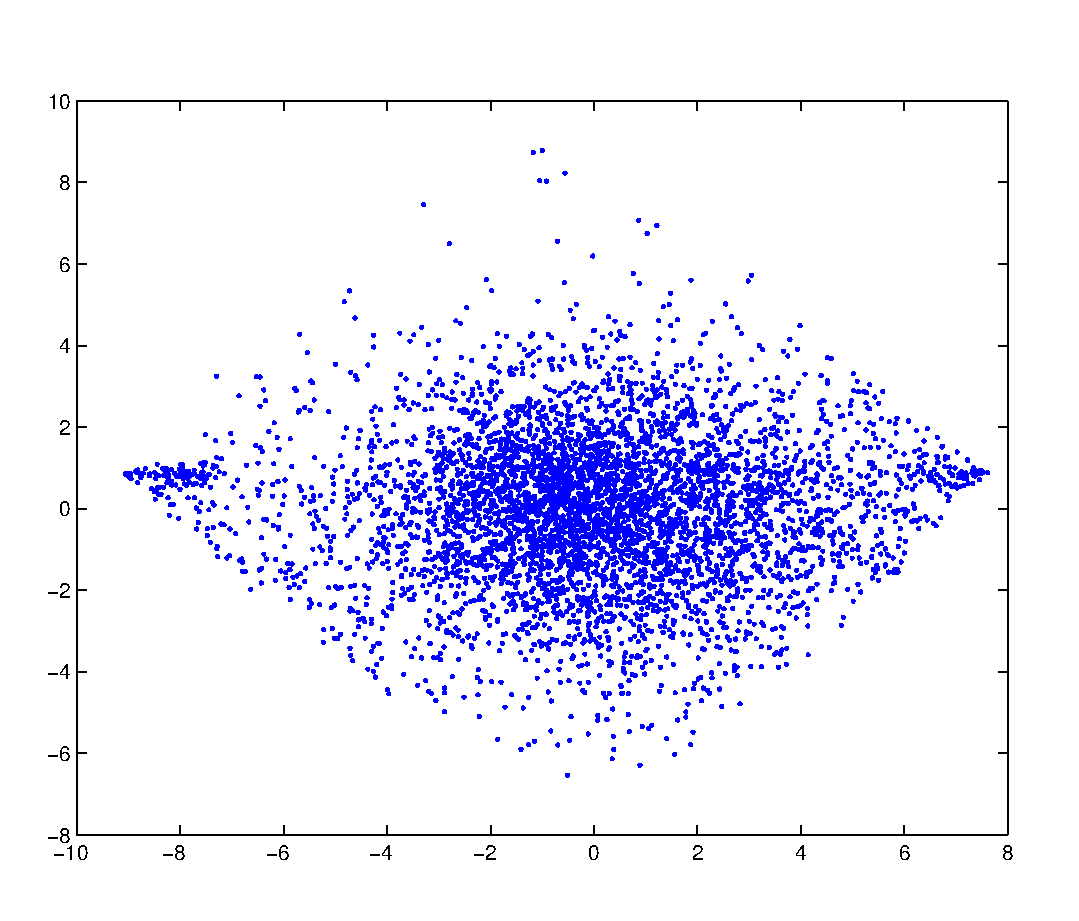
\includegraphics[width=\linewidth]{eigentaste_proj_cropped.pdf}
	}
	\frame[plain]{
		\frametitle{Choix du nombre de clusters}
		\centering
		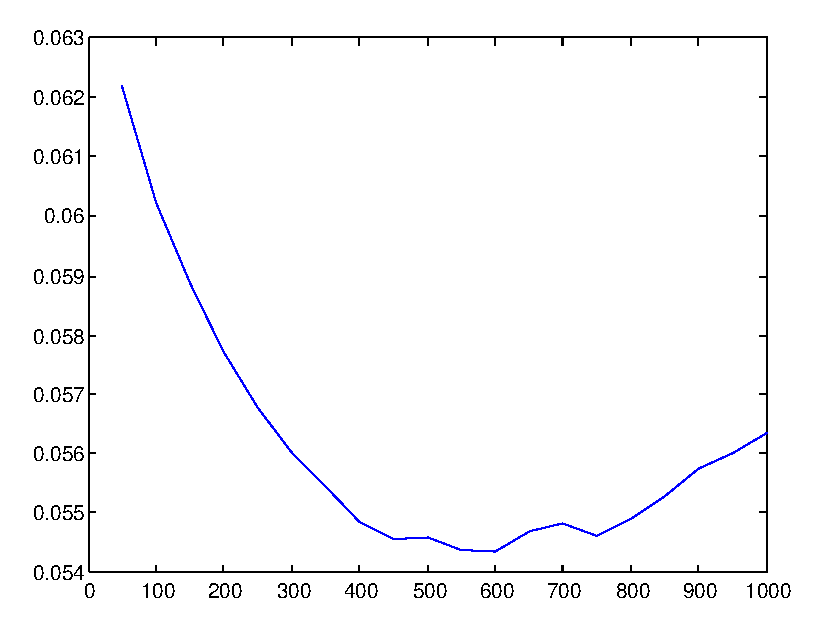
\includegraphics[width=0.4\linewidth]{optimalMaxClust01_cropped.pdf}
		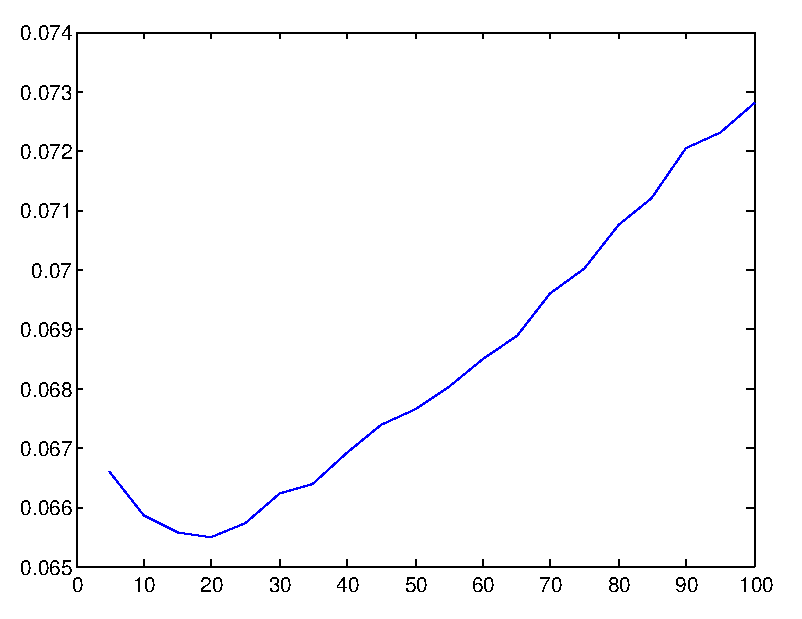
\includegraphics[width=0.4\linewidth]{optimalMaxClust02_cropped.pdf}
	}
	
	\frame[plain]{
		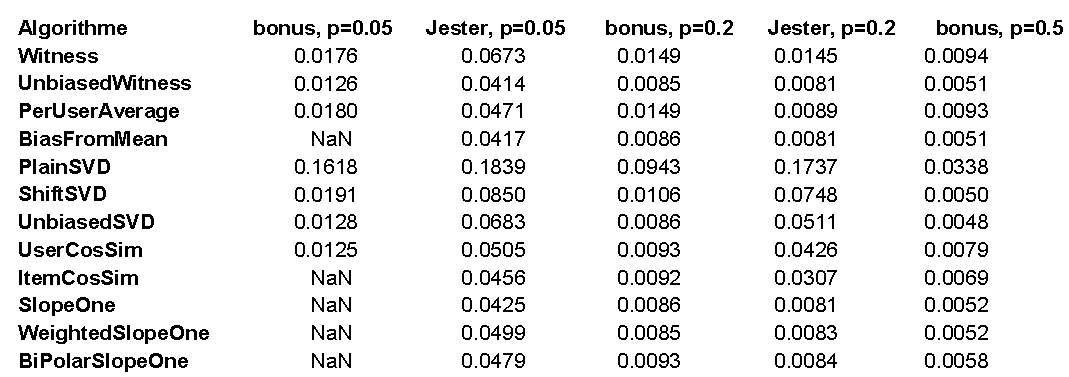
\includegraphics[width=\linewidth]{resultatsRapport_cropped.pdf}
		
		Jeux de données : \begin{itemize}
			\item Matrice de la question bonus du DM
			\item Jester : ensemble de ratings d'une centaine de blagues par plus de $50000$ utilisateurs, avec un sous-ensemble noté par tout le monde
		\end{itemize}
	}
	\frame[plain]{
		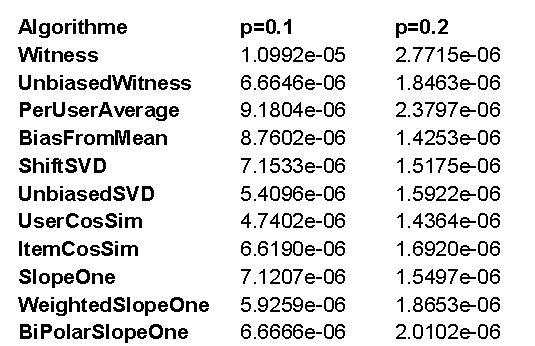
\includegraphics[width=\linewidth]{MAE_cropped.pdf}
	}
	\frame[plain]{
		\frametitle{Bilan}
		\begin{itemize}
			\item Selon le jeu de données et l'objectif (norme d'erreur), le choix de l'algorithme est très variable
			\item Compromis à faire entre précision, temps de calcul, mémoire, vitesse des requêtes et des mises à jour
		\end{itemize}
		}
\end{document}

